\documentclass[conference]{IEEEtran}

% ── Packages ──────────────────────────────────────────────────────────────────
\usepackage[T1]{fontenc}
\usepackage[utf8]{inputenc}
\usepackage{amsmath,amssymb}
\usepackage{graphicx}
\usepackage{booktabs}
\usepackage{array}
\usepackage{cite}
\usepackage{url}
\usepackage{hyperref}
\usepackage{tikz}
\usetikzlibrary{positioning,arrows.meta,shapes.geometric,calc,patterns}
\usepackage{pgfplots}
\pgfplotsset{compat=1.18}
\usepackage{float}
\usepackage{microtype}
% algorithm packages not available; using manual pseudocode
\usepackage{multirow}
\usepackage{tabularx}

% ── Title & Authors ───────────────────────────────────────────────────────────
\title{MycoFlow: A Bio-Inspired, Reflexive QoS System\\
       for Embedded OpenWrt Routers}

\author{
  \IEEEauthorblockN{Bar\i{}s Can Atakl\i{}}
  \IEEEauthorblockA{Department of Software Engineering\\
    Mu\u{g}la S\i{}tk\i{} Ko\c{c}man University\\
    Mu\u{g}la, Turkey\\
    baris.atakli@ogr.mu.edu.tr}
  \and
  \IEEEauthorblockN{Dr.\ \"{O}\u{g}r.\ \"{U}yesi Cihat \c{C}etinkaya}
  \IEEEauthorblockA{Department of Software Engineering\\
    Mu\u{g}la S\i{}tk\i{} Ko\c{c}man University\\
    Mu\u{g}la, Turkey}
}

\begin{document}

\maketitle

% ─────────────────────────────────────────────────────────────────────────────
% ABSTRACT
% ─────────────────────────────────────────────────────────────────────────────
\begin{abstract}
Consumer home networks must simultaneously serve latency-sensitive workloads
(online gaming, VoIP, video conferencing) and high-throughput bulk transfers
(streaming, torrents, backups) on commodity routers with tight CPU, RAM, and
flash constraints.
Static queue management strategies, even when combined with modern Active
Queue Management (AQM) algorithms such as CAKE, cannot automatically classify
encrypted, mixed-application traffic at the per-device level or adapt bandwidth
caps to real-time congestion signals.
We present \emph{MycoFlow}, a bio-inspired, fully embedded Quality-of-Service
daemon for OpenWrt routers that draws its design principles from the adaptive
resource-allocation behavior of fungal mycelial networks.
MycoFlow operates a 1~Hz Sense$\to$Infer$\to$Act$\to$Stabilize reflexive loop
entirely on-device and classifies traffic on two complementary levels.
The device level assigns each LAN host one of six behavioral personas;
the flow level assigns each conntrack 5-tuple one of twelve service classes
(game\_rt, voip\_call, video\_conf, video\_vod, bulk\_dl, torrent, etc.)
using a three-signal weighted voter that combines passive DNS snooping,
destination-port hints, and behavioral fingerprints (packet size, throughput,
reverse-byte ratio).
Classified flows receive a conntrack mark which is translated to a DSCP
value in the mangle POSTROUTING chain, steering them into CAKE diffserv
priority tins.
A passive BPF TCP RTT observer, attached at the TC egress and ingress hooks,
feeds a per-flow round-trip smoothed estimate to an auto-corrector that
demotes a flow one tier when its RTT exceeds the class target by 50\,\% for
two consecutive cycles, and re-promotes it symmetrically.
A feedback-driven hysteresis controller adjusts the WAN bandwidth cap;
all learning state is RAM-resident, so the daemon writes zero bytes to the
router's NAND flash.
Three controlled experiments demonstrate:
(i)~a \textbf{154$\times$ lower average in-tin delay} for gaming traffic
vs.\ bulk traffic when per-device DSCP marking is active;
(ii)~a \textbf{38\% reduction in gaming latency} under five simultaneous
mixed-persona clients compared to CAKE-only AQM; and
(iii)~correct per-flow service separation when a single source IP
simultaneously runs interactive, bulk, and torrent-style workloads---the
failure case that per-device classification cannot resolve.
The daemon runs within a $<$2\% CPU budget on the target Xiaomi~AX3000T
(MediaTek~MT7981B, 256~MB~RAM) and is packaged as a standard OpenWrt IPK
now deployed on a live home-network router.
\end{abstract}

\begin{IEEEkeywords}
bufferbloat, CAKE, DSCP, eBPF, OpenWrt, persona-aware QoS, reflexive control,
bio-inspired networking, home network, adaptive queue management,
flow-aware classification, passive TCP RTT, conntrack, CONNMARK, service
taxonomy
\end{IEEEkeywords}

% ─────────────────────────────────────────────────────────────────────────────
% I. INTRODUCTION
% ─────────────────────────────────────────────────────────────────────────────
\section{Introduction}

The modern household router is the single most critical network device
for millions of users, yet it typically operates a fixed, administrator-configured
Quality of Service (QoS) policy that was set at install time and never updated.
Meanwhile, the application mix on a home network changes continuously:
a gaming session demands sub-5~ms latency, a video conference requires
stable 200--400~kbps with jitter below 15~ms, a streaming client needs
8--25~Mbps with no packet loss, and a background BitTorrent process competes for
any remaining bandwidth with hundreds of simultaneous TCP connections.

\textbf{Bufferbloat}~\cite{gettys2012}—the phenomenon where excess queuing
inside network devices inflates round-trip time by hundreds of milliseconds—
remains the dominant cause of degraded user experience on home networks.
A single saturating TCP flow can fill a 1000-packet FIFO queue in under
100~ms on a 20~Mbit/s WAN link, rendering gaming and VoIP completely
unusable until the flow terminates.

Active Queue Management (AQM) algorithms such as
CoDel~\cite{nichols2012}, fq\_CoDel~\cite{hoeiland2018}, and
CAKE~\cite{cake2018} have made significant progress against bufferbloat.
CAKE in particular, which is the default AQM on OpenWrt since version~22.03,
combines shaping, per-flow fair queuing, and Differentiated Services (DiffServ)
priority tins in a single qdisc.
However, two fundamental challenges remain unsolved for home deployments:

\begin{itemize}
  \item \textbf{No automatic traffic classification.} CAKE's diffserv mode
    relies on DSCP markings in IP headers. On home networks, most traffic
    arrives with CS0 (Best~Effort) markings, so every flow—gaming, streaming,
    torrent—lands in the same tin regardless of its latency sensitivity.
  \item \textbf{Static WAN rate limit.} The CAKE bandwidth parameter is set
    once. It cannot react to congestion detected through probe-based
    measurements or queue depth signals.
\end{itemize}

We present \textbf{MycoFlow}, a lightweight C11 daemon that addresses both
problems.
Its design is inspired by the information-processing strategy of fungal
mycelial networks~\cite{fricker2017mycelium}: a mycelium continuously senses
its environment through hyphal tip probes, redistributes nutrients adaptively
using hysteresis-controlled transport decisions, and restructures itself in
response to persistent stress.
MycoFlow translates these principles to the network control plane: periodic
probe-based sensing, per-device persona inference from flow statistics,
DSCP-based traffic steering into CAKE tins, and bandwidth adaptation governed
by a hysteresis controller with sliding baseline tracking.

\textbf{Contributions of this paper:}
\begin{enumerate}
  \item A six-class per-device traffic persona engine that infers application
    category (VOIP, GAMING, VIDEO, STREAMING, BULK, TORRENT) from conntrack
    flow statistics without deep-packet inspection or machine learning.
  \item A twelve-class per-flow service taxonomy (game\_rt, voip\_call,
    video\_conf, video\_live, video\_vod, web\_interactive, bulk\_dl,
    file\_sync, torrent, game\_launcher, system, unknown) classified by a
    three-signal weighted voter that combines passive DNS snooping (0.6),
    destination-port hints (0.3), and behavioral fingerprints (0.1), with a
    two-tick stability gate before marking is applied.
  \item A CONNMARK-based per-flow DSCP pipeline: once the classifier commits a
    decision, a libnetfilter\_conntrack update writes a service tag into the
    flow's conntrack mark, and an nftables mangle POSTROUTING chain restores
    the mark to DSCP on every egress packet of that 5-tuple.
  \item A passive TCP~RTT observer implemented as a BPF program attached at
    the TC~clsact egress and ingress hooks on the WAN interface, populating a
    per-flow RTT map consulted by an auto-corrector that demotes a flow one
    service tier when smoothed RTT exceeds the class target by 50\% for two
    consecutive cycles, and re-promotes it symmetrically.
  \item A formal reflexive control loop with EWMA smoothing, adaptive
    congestion thresholds scaled to per-link baselines, and a sliding EWMA
    baseline that tracks long-term idle conditions.
  \item An action feedback ring that detects ineffective bandwidth adjustments
    and halves the step size automatically, preventing controller oscillation.
  \item A reproducible three-phase QEMU/Docker evaluation covering 2-persona,
    6-persona, and single-IP multi-app workloads, with detailed CAKE tin
    statistics, per-device classification, and per-flow service separation
    results.
  \item A production-ready OpenWrt package with UCI configuration, procd init
    integration, LuCI dashboard (including a per-flow service table with
    live demote indicators), and zero flash writes during operation---now
    deployed on a live Xiaomi~AX3000T home router.
\end{enumerate}

The remainder of this paper is organized as follows.
Section~\ref{sec:background} provides background on bufferbloat and AQM.
Section~\ref{sec:related} surveys related work.
Section~\ref{sec:bio} explains the bio-inspired design rationale.
Section~\ref{sec:architecture} presents the system architecture.
Section~\ref{sec:control} formalizes the control loop.
Section~\ref{sec:impl} describes the implementation.
Section~\ref{sec:eval} reports evaluation results.
Section~\ref{sec:discussion} discusses implications and limitations.
Section~\ref{sec:conclusion} concludes.

% ─────────────────────────────────────────────────────────────────────────────
% II. BACKGROUND
% ─────────────────────────────────────────────────────────────────────────────
\section{Background}
\label{sec:background}

\subsection{Bufferbloat and AQM}

When a WAN uplink is saturated, the router's transmit queue accumulates
packets faster than they can be sent.
Without queue management, packets wait in FIFO order; round-trip time grows
linearly with queue depth.
On a 20~Mbit/s uplink with a 1000-packet queue and 1500-byte packets, the
maximum queue drain time exceeds 600~ms—far beyond the 20~ms threshold for
interactive applications.

CoDel~\cite{nichols2012} controls standing queue depth by measuring the
minimum queuing delay experienced by packets over a sliding window;
it signals congestion via ECN or drops when the minimum delay exceeds
a target (typically 5~ms) for longer than an interval (100~ms).
fq\_CoDel~\cite{hoeiland2018} adds per-flow fair queuing so that a single
bulk flow cannot monopolize the queue at the expense of interactive flows.
CAKE~\cite{cake2018} subsumes both and adds three layers of priority:
per-tin bandwidth allocation, per-flow isolation within each tin, and
per-host round-robin within each flow set.

\subsection{CAKE diffserv4}

CAKE's \texttt{diffserv4} mode partitions traffic into four tins based on
the IP Precedence field (upper three bits of DSCP):
Voice (Precedence 4--7), Video (Precedence 2--3), Best~Effort (Precedence 0),
and Bulk (Precedence 1).
Each tin has an independent minimum guaranteed rate and an AQM target delay.
Under CAKE diffserv4, a packet with DSCP CS4 (Precedence 4) enters the Voice
tin and is served before any Best~Effort or Bulk packet.
MycoFlow exploits this mechanism: by correctly marking per-device flows,
it shifts traffic from the default Best~Effort tin into the appropriate
priority tier without any modification to CAKE itself.

The DSCP-to-tin mapping used by MycoFlow is:
EF $\to$ Voice (VoIP),
CS4 $\to$ Voice (gaming),
CS3 $\to$ Video (video call),
CS2 $\to$ Video (streaming),
CS1 $\to$ Bulk (torrent, bulk transfer).

\subsection{DiffServ and DSCP on Home Networks}

The Differentiated Services architecture~\cite{rfc2474} defines
per-hop behaviors based on the DSCP field of the IP header.
Edge routers are expected to re-mark traffic entering the network, but most
ISP CPE devices either ignore DSCP or clear it.
Home devices typically generate unmarked traffic (CS0), and no mechanism
exists to automatically reclassify it at the home gateway.
MycoFlow fills this gap by inferring intent from behavioral signals rather
than port numbers or payload inspection.

% ─────────────────────────────────────────────────────────────────────────────
% III. RELATED WORK
% ─────────────────────────────────────────────────────────────────────────────
\section{Related Work}
\label{sec:related}

\textbf{AQM evolution.}
Proportional Integral controller Enhanced (PIE)~\cite{pan2013pie} achieves
CoDel-equivalent performance with lower computational cost.
FQ-PIE combines PIE with per-flow queuing.
CAKE~\cite{cake2018} remains the most comprehensive open-source AQM
for home gateways, integrating shaping, fair queuing, and DiffServ.
None of these systems perform automatic per-device DSCP classification.

\textbf{Traffic classification.}
DeepFlow~\cite{zhao2023} applies a lightweight CNN to encrypted traffic
classification; it achieves high accuracy but requires GPU inference and
cloud-side model updates, making it incompatible with embedded routers.
ACAS~\cite{lotfollahi2020deep} uses deep learning on raw packet features;
again, resource requirements preclude embedded deployment.
nDPI~\cite{ndpi2022} provides open-source DPI classification but requires
payload parsing, raising privacy concerns and significant CPU cost on
constrained hardware.
MycoFlow deliberately avoids both ML and DPI: its heuristic decision tree
runs in under 1~$\mu$s per device per cycle on a Cortex-A53 core.

\textbf{Adaptive QoS.}
Tang and Yu~\cite{tang2024} propose SDN-based per-application QoS for home
networks; their approach requires a controller external to the CPE.
OpenWrt \texttt{qosify} provides static DSCP mapping via nftables rules
with fixed port-to-class tables, but no runtime sensing or adaptation.
SQM (Smart Queue Management) in OpenWrt configures CAKE or fq\_CoDel with
appropriate parameters but does not adapt them during operation.
Nichols et al.~\cite{nichols2024} discuss CAKE extensions for diffserv
auto-learning; this work is complementary to MycoFlow and could in principle
replace the manual DSCP marking with kernel-level auto-classification.

\textbf{eBPF for edge telemetry.}
Popescu et al.~\cite{popescu2024} demonstrate the use of eBPF telemetry maps
for adaptive metrics on edge routers, showing that kernel-side counters can
expose per-flow statistics with negligible overhead.
MycoFlow uses eBPF for packet-rate counting via a TC hook but primarily
relies on \texttt{/proc/net/nf\_conntrack} for flow statistics, as eBPF
kernel headers are not available on all OpenWrt builds.

\textbf{Bio-inspired networking.}
Ant Colony Optimization~\cite{dorigo1996ant} has been applied to routing
in multi-hop networks but requires agent communication infrastructure
absent in home routers.
Adamatzky and colleagues~\cite{adamatzky2022logics} characterize mycelial
networks as fault-tolerant distributed logic gates.
Fricker et al.~\cite{fricker2017mycelium} model nutrient transport in
mycelial networks as an adaptive flow optimization problem.
Fukasawa et al.~\cite{fukasawa2023foraging} analyze how foraging heuristics
in mycelium maximize resource extraction under uncertainty.
MycoFlow is the first system to apply mycelial foraging and transport
principles specifically to the QoS control plane of an embedded router.

\textbf{Positioning.}
MycoFlow occupies a unique design point: it runs \emph{entirely on the CPE},
requires \emph{no cloud or SDN controller}, uses \emph{no ML or DPI},
and \emph{automatically classifies and steers} per-device traffic.
Table~\ref{tab:comparison} summarizes the comparison.

\begin{table}[t]
\caption{Comparison of Related QoS Approaches}
\label{tab:comparison}
\centering
\small
\begin{tabular}{p{1.8cm}ccccc}
\toprule
\textbf{System} & \textbf{Emb.} & \textbf{Auto} & \textbf{No ML} & \textbf{No DPI} & \textbf{Adapt} \\
\midrule
SQM/CAKE     & \checkmark & $\times$ & \checkmark & \checkmark & $\times$ \\
qosify       & \checkmark & $\times$ & \checkmark & $\times$   & $\times$ \\
nDPI         & $\times$   & \checkmark & \checkmark & $\times$ & $\times$ \\
DeepFlow     & $\times$   & \checkmark & $\times$   & \checkmark & $\times$ \\
SDN-QoS      & $\times$   & \checkmark & \checkmark & \checkmark & \checkmark \\
\textbf{MycoFlow} & \checkmark & \checkmark & \checkmark & \checkmark & \checkmark \\
\bottomrule
\end{tabular}
\end{table}

% ─────────────────────────────────────────────────────────────────────────────
% IV. BIO-INSPIRED DESIGN RATIONALE
% ─────────────────────────────────────────────────────────────────────────────
\section{Bio-Inspired Design Rationale}
\label{sec:bio}

Mycelial networks solve a resource allocation problem structurally identical to
home network QoS: a single nutrient source (the WAN uplink) must be distributed
among competing consumers (devices and applications) with heterogeneous
latency requirements, under dynamic and partially observable conditions.

Mycelium achieves this through four mechanisms that map directly to
MycoFlow's design (Table~\ref{tab:bio}):

\begin{table}[t]
\caption{Mycelial Principles Mapped to MycoFlow}
\label{tab:bio}
\centering
\small
\begin{tabular}{p{2.0cm}p{5.6cm}}
\toprule
\textbf{Biology} & \textbf{MycoFlow Mechanism} \\
\midrule
Hyphal tip sensing & ICMP multi-ping probes; Netlink qdisc stats; eBPF packet counters \\
Adaptive nutrient redistribution & Per-device DSCP marking into CAKE priority tins \\
Hysteresis \& structural memory & Majority-vote history window; stable-state snapshots; action cooldown timers \\
Mycelial network remodeling & Sliding EWMA baseline; bandwidth step adaptation via action feedback ring \\
\bottomrule
\end{tabular}
\end{table}

The key property borrowed from mycelial biology is \emph{local decision-making}:
each routing decision in a mycelium depends only on local chemical gradients,
not on a global network map.
MycoFlow similarly requires no external state: all classification and control
decisions derive from metrics collected on the router itself.

The mycelial analogy also motivates the choice of hysteresis as the primary
stability mechanism.
Mycelial networks do not oscillate between resource allocation states because
transport channels have inertia: they require a sustained signal above a
threshold before remodeling occurs.
MycoFlow's $k$-of-$m$ majority vote (default $k=3$, $m=5$ cycles) and
cooldown timers serve the same purpose.

% ─────────────────────────────────────────────────────────────────────────────
% V. SYSTEM ARCHITECTURE
% ─────────────────────────────────────────────────────────────────────────────
\section{System Architecture}
\label{sec:architecture}

\subsection{Overview}

MycoFlow consists of five components deployed on the OpenWrt router:
\texttt{mycoflowd} (the control daemon), a CAKE qdisc on the WAN interface,
an optional CAKE qdisc on an IFB device for ingress shaping, an iptables mangle
chain for DSCP marking, and the LuCI dashboard.

Fig.~\ref{fig:arch} shows the reflexive loop.
The daemon runs at a configurable rate (default 1~Hz) and executes four
phases per cycle:

\begin{enumerate}
  \item \textbf{Sense:} Collect RTT/jitter via ICMP probes, interface
    byte/packet counters via \texttt{/proc/net/dev}, qdisc statistics
    via NETLINK\_ROUTE, and flow statistics from
    \texttt{/proc/net/nf\_conntrack}.
  \item \textbf{Infer:} Apply EWMA smoothing to raw metrics; run the
    six-class per-device persona engine; update the system-wide persona
    via majority vote.
  \item \textbf{Act:} If the persona changed, update CAKE AQM target latency
    and apply per-device DSCP mangle rules. If congestion is detected, adjust
    the WAN bandwidth cap subject to cooldown constraints.
  \item \textbf{Stabilize:} Record actuation outcomes in the feedback ring;
    evaluate ring for step-size adaptation; update the sliding baseline.
\end{enumerate}

\begin{figure}[t]
\centering
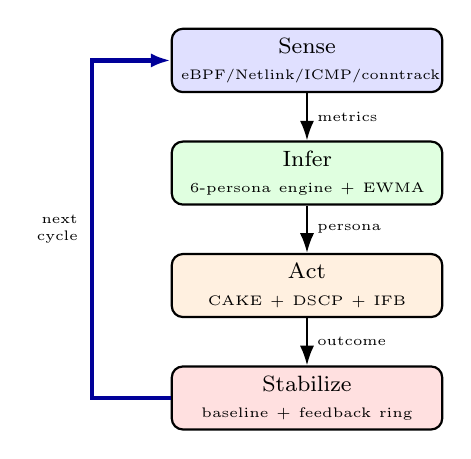
\begin{tikzpicture}[
  node distance=0.6cm and 0.3cm,
  blk/.style={draw, thick, rounded corners, minimum height=0.80cm,
              text width=3.2cm, align=center, font=\footnotesize},
  arr/.style={-{Latex[length=2.5mm,width=1.8mm]}, thick}
]
\node[blk, fill=blue!12]   (sense)  {Sense\\{\tiny eBPF/Netlink/ICMP/conntrack}};
\node[blk, fill=green!12,  below=of sense]  (infer)  {Infer\\{\tiny 6-persona engine + EWMA}};
\node[blk, fill=orange!12, below=of infer]  (act)    {Act\\{\tiny CAKE + DSCP + IFB}};
\node[blk, fill=red!12,    below=of act]    (stab)   {Stabilize\\{\tiny baseline + feedback ring}};

\draw[arr] (sense.south) -- node[right,font=\tiny]{metrics}  (infer.north);
\draw[arr] (infer.south) -- node[right,font=\tiny]{persona}  (act.north);
\draw[arr] (act.south)   -- node[right,font=\tiny]{outcome}  (stab.north);

\coordinate (lbot) at ($(stab.west)+(-1.0,0)$);
\coordinate (ltop) at ($(sense.west)+(-1.0,0)$);
\draw[arr, draw=blue!60!black, ultra thick]
  (stab.west) -- (lbot) --
  node[left,font=\tiny,xshift=-1pt,align=right]{next\\cycle}
  (ltop) -- (sense.west);
\end{tikzpicture}
\caption{MycoFlow reflexive control loop.}
\label{fig:arch}
\end{figure}

\subsection{Module Structure}

The daemon comprises 20~C11 source modules (Table~\ref{tab:modules})
totalling approximately 4\,500~lines of code, compiled for
\texttt{aarch64-openwrt-linux-musl} via the OpenWrt~SDK.
The modules are grouped into three layers: (i)~the core 1~Hz reflexive
loop, (ii)~the per-device persona layer, and (iii)~the v3 flow-aware
layer (classifier, mark engine, passive RTT observer) that classifies
individual conntrack 5-tuples into service classes.

\begin{table}[t]
\caption{MycoFlow Source Modules and Responsibilities}
\label{tab:modules}
\centering
\small
{\setlength{\tabcolsep}{4pt}
\begin{tabular}{p{2.2cm}p{5.4cm}}
\toprule
\textbf{Module} & \textbf{Responsibility} \\
\midrule
\multicolumn{2}{l}{\emph{Core reflexive loop}} \\
\texttt{myco\_sense}      & ICMP multi-ping, \texttt{/proc/net/dev}, CPU \\
\texttt{myco\_control}    & EWMA, adaptive thresholds, feedback ring \\
\texttt{myco\_act}        & \texttt{tc}/\texttt{iptables} actuation, IFB \\
\texttt{myco\_ewma}       & Generic EWMA filter \\
\texttt{myco\_netlink}    & NETLINK\_ROUTE qdisc statistics \\
\texttt{myco\_ebpf}       & BPF map reading, TC hook management \\
\texttt{myco\_config}     & UCI + environment + compiled defaults \\
\texttt{myco\_ubus}       & ubus IPC + \texttt{/tmp/myco\_state.json} \\
\texttt{myco\_log}        & Structured stdout logging \\
\midrule
\multicolumn{2}{l}{\emph{Per-device persona layer}} \\
\texttt{myco\_persona}    & 6-class decision tree, majority-vote window \\
\texttt{myco\_flow}       & LRU conntrack table, elephant detection \\
\texttt{myco\_device}     & Per-device persona table, DSCP rules \\
\midrule
\multicolumn{2}{l}{\emph{Flow-aware v3 layer}} \\
\texttt{myco\_service}    & 12-class service taxonomy + demote ladder \\
\texttt{myco\_hint}       & Destination-port hint table \\
\texttt{myco\_dns}        & Passive DNS snooping cache (name$\to$IP) \\
\texttt{myco\_profile}    & Per-flow behavioral fingerprint \\
\texttt{myco\_classifier} & 3-signal weighted voter + stability gate \\
\texttt{myco\_mark}       & \texttt{libnetfilter\_conntrack} CT-mark push \\
\texttt{myco\_mangle}     & nftables mangle POSTROUTING DSCP restore \\
\texttt{myco\_rtt}        & libbpf TC-clsact passive TCP RTT observer \\
\bottomrule
\end{tabular}}
\end{table}

% ─────────────────────────────────────────────────────────────────────────────
% VI. THE CONTROL LOOP
% ─────────────────────────────────────────────────────────────────────────────
\section{The Control Loop}
\label{sec:control}

\subsection{Metric Sensing and Smoothing}

\textbf{RTT and jitter.}
Every cycle, \texttt{myco\_sense} issues three ICMP echo requests to a
configurable probe host (default \texttt{1.1.1.1}), measuring mean RTT
and standard deviation (jitter) from the replies.
Packet loss is computed as $(N_{\rm sent} - N_{\rm received})/N_{\rm sent}$.
Raw measurements are smoothed by an Exponentially Weighted Moving Average
(EWMA) with parameter $\alpha$:
\begin{equation}
  \hat{r}_t = \alpha\, r_t + (1-\alpha)\,\hat{r}_{t-1}, \quad
  \hat{j}_t = \alpha\, j_t + (1-\alpha)\,\hat{j}_{t-1}.
  \label{eq:ewma}
\end{equation}
The default $\alpha = 0.30$ provides a time constant of approximately
3~cycles (3~s at 1~Hz), balancing responsiveness and noise rejection.

\textbf{Queue statistics.}
A raw NETLINK\_ROUTE socket (RTM\_GETQDISC) retrieves the CAKE qdisc's
\texttt{backlog} (bytes queued), \texttt{drops}, and \texttt{overlimits}
each cycle.
A non-zero backlog is a direct kernel-side bufferbloat indicator,
faster and more reliable than the RTT probe alone.

\textbf{Flow statistics.}
\texttt{myco\_flow} parses \texttt{/proc/net/nf\_conntrack} into a
userspace LRU hash table (256~entries, FNV-1a hash).
For each entry, both forward (src$\to$dst) and reverse (dst$\to$src) byte
counts are extracted; the reverse direction carries download volume,
which is essential for distinguishing STREAMING (high rx, low tx) from BULK
(high rx, high tx).
Stale entries (no activity for 60~s) are evicted each cycle.
An \emph{elephant flow} is defined as a single flow carrying more than 60\%
of a device's total bytes.

\subsection{Six-Persona Classification Engine}

\texttt{myco\_device} maintains a per-device record keyed by \texttt{src\_ip}.
Each cycle, flows from the conntrack table are aggregated per source IP,
and the device's behavioral profile is updated: total active flows, total
bytes, reverse bytes, average packet size, and elephant flow flag.

The six personas are inferred via the priority-ordered decision tree in
Algorithm~\ref{alg:persona}.
A three-of-five majority vote over a sliding history window prevents
rapid class oscillation: only when a persona wins in at least 3 of the
5 most recent cycles does it become the device's current class.

\begin{figure}[t]
\centering
\small
\begin{tabular}{p{0.42\columnwidth}p{0.49\columnwidth}}
\toprule
\textbf{Condition (priority order)} & \textbf{Persona} \\
\midrule
$F > 30$ & \textsc{Torrent} \\
$E$ and $B_{rx}/B < 0.25$ & \textsc{Streaming} \\
$E$ & \textsc{Bulk} \\
$\bar{s} < 120$\,B and $\dot{B} < 200$\,kbps & \textsc{Voip} \\
$\bar{s} < 350$\,B and $F < 8$ & \textsc{Gaming} \\
$200\,\text{kbps} \le \dot{B} \le 8\,\text{Mbps}$ & \textsc{Video} \\
otherwise & \textsc{Unknown} \\
\bottomrule
\multicolumn{2}{l}{\footnotesize $F$: flows; $E$: elephant flag; $B_{rx}$: reverse bytes;} \\
\multicolumn{2}{l}{\footnotesize $\bar{s}$: avg pkt size; $\dot{B}$: device throughput.} \\
\end{tabular}
\caption{Persona inference decision table (first matching rule wins).}
\label{alg:persona}
\end{figure}

Each persona maps to a DSCP value enforced by an iptables mangle rule in
the \texttt{mycoflow\_dscp} chain (Table~\ref{tab:dscpmap}).
When a device's persona changes, the old rule is removed and a new rule
is inserted atomically.
\begin{table}[t]
\caption{Persona-to-DSCP-to-CAKE-Tin Mapping}
\label{tab:dscpmap}
\centering
\small
\begin{tabular}{llcl}
\toprule
\textbf{Persona} & \textbf{DSCP} & \textbf{Prec.} & \textbf{CAKE Tin} \\
\midrule
VOIP      & EF   & 6 & Voice      \\
GAMING    & CS4  & 4 & Voice      \\
VIDEO     & CS3  & 3 & Video      \\
STREAMING & CS2  & 2 & Video      \\
BULK      & CS1  & 1 & Bulk       \\
TORRENT   & CS1  & 1 & Bulk       \\
UNKNOWN   & CS0  & 0 & Best Effort\\
\bottomrule
\end{tabular}
\end{table}

\subsection{Flow-Aware Service Classification (v3)}
\label{subsec:flowaware}

The per-device persona layer delivers correct behavior when each LAN host
runs a single dominant application, but collapses when one source~IP
simultaneously carries a video call, a bulk download, and a torrent
swarm: a single persona must be chosen for all of them, and three
quarters of the traffic is mis-classified.
MycoFlow~v3 adds a second classification axis that operates on individual
conntrack 5-tuples.

\textbf{Service taxonomy.}
Twelve service classes (Table~\ref{tab:services}) cover the traffic
types commonly seen on home links.
Each class carries a target RTT, a default DSCP mark, and a demotion
successor used by the RTT auto-corrector.
When a flow's measured RTT persistently exceeds its target, it walks
one step down the ladder (e.g., \textsc{game\_rt} $\to$
\textsc{web\_interactive} $\to$ \textsc{bulk\_dl}).

\begin{table}[t]
\caption{Flow-Level Service Taxonomy}
\label{tab:services}
\centering
\scriptsize
{\setlength{\tabcolsep}{3pt}
\begin{tabular}{llrl}
\toprule
\textbf{Service} & \textbf{DSCP} & \textbf{Target RTT} & \textbf{Demotes to} \\
\midrule
game\_rt          & EF   & 20~ms  & web\_interactive \\
voip\_call        & EF   & 30~ms  & web\_interactive \\
video\_conf       & CS4  & 50~ms  & web\_interactive \\
video\_live       & CS3  & 100~ms & bulk\_dl \\
video\_vod        & CS2  & 150~ms & bulk\_dl \\
web\_interactive  & CS2  & 80~ms  & bulk\_dl \\
game\_launcher    & CS1  & 200~ms & bulk\_dl \\
file\_sync        & CS1  & 200~ms & bulk\_dl \\
bulk\_dl          & CS1  & 250~ms & torrent \\
torrent           & CS1  & 400~ms & torrent \\
system            & CS0  & ---    & unknown \\
unknown           & CS0  & ---    & unknown \\
\bottomrule
\end{tabular}}
\end{table}

\textbf{Three-signal weighted voter.}
For every active conntrack entry, \texttt{myco\_classifier} produces a
score for each candidate service by summing three independently
normalized signals:
\begin{equation}
  S_c(f) = w_{\rm dns}\,D_c(f) + w_{\rm port}\,P_c(f) + w_{\rm behav}\,B_c(f),
  \label{eq:voter}
\end{equation}
with weights $(w_{\rm dns}, w_{\rm port}, w_{\rm behav}) = (0.6, 0.3, 0.1)$
and an acceptance threshold $\theta = 0.3$.
$D_c(f)$ is computed from a passive DNS snooping cache that records,
for each resolved name, the set of services its suffix pattern matches
(e.g.\ \texttt{discord.gg} $\to$ \textsc{voip\_call}).
$P_c(f)$ consults a destination-port hint table (e.g.\ UDP/3478 STUN $\to$
\textsc{voip\_call}, UDP/27015 Source-engine $\to$ \textsc{game\_rt}).
$B_c(f)$ is a behavioral fingerprint from \texttt{myco\_profile}: mean
packet size, packets-per-second, inter-arrival jitter, and burstiness.
The class with the highest score above $\theta$ wins; otherwise the
flow remains \textsc{unknown} and is re-evaluated next cycle.

\textbf{Stability gate.}
A decision is committed only after it has been observed in two
consecutive ticks ($\approx 1$~s at 2~Hz).
This suppresses oscillation from short flows (DNS queries, TCP
handshakes) that never accumulate enough signal to justify a mark.

\textbf{CONNMARK push and DSCP restore.}
Once a flow is stable, \texttt{myco\_mark} issues an
\texttt{NFCT\_Q\_UPDATE} via \texttt{libnetfilter\_conntrack} to set
the conntrack entry's mark to the service tag.
An nftables mangle chain in \texttt{POSTROUTING} restores this mark
to DSCP on every egress packet, so per-flow differentiation survives
across the full lifetime of the connection without kernel-side
classifier programs.

\textbf{RTT auto-corrector.}
\texttt{myco\_rtt} loads a BPF program onto the TC~clsact egress and
ingress hooks of the WAN interface.
For each TCP flow, the BPF program samples the TSval/TSecr pair from
the TCP timestamp option and records the elapsed time, maintaining a
smoothed per-flow RTT in a BPF hash map.
The userspace classifier polls this map each tick.
If a flow's smoothed RTT exceeds its service's target by more than
50\% for two consecutive ticks, the flow is demoted one tier and a
new CT~mark is written; if the RTT recovers below the target for
two ticks, it is re-promoted symmetrically.
A \texttt{demoted} bit is exported in the JSON state so the LuCI
dashboard can render an indicator next to the service badge.

\subsection{Congestion Detection and Bandwidth Policy}

\textbf{Adaptive thresholds.}
Let $\mathcal{L}=\{\text{VOIP, GAMING, VIDEO}\}$ (latency-sensitive) and
$\mathcal{B}=\{\text{BULK, STREAMING, TORRENT}\}$ (bulk-tolerant).
Congestion is declared when any of the following conditions hold:
\begin{align}
  \hat{r}_t &> r_{\rm base}\cdot(1+\gamma) \label{eq:rtt_cong}\\
  \hat{j}_t &> j_{\rm base}\cdot(1+\gamma) \label{eq:jit_cong}\\
  \text{backlog}_t &> 0 \label{eq:bl_cong}\\
  \ell_t &> 0.02 \label{eq:loss_cong}
\end{align}
where $r_{\rm base}$, $j_{\rm base}$ are the sliding baselines
(Section~\ref{subsec:baseline}), $\gamma=0.30$ is the margin factor
(tunable), and $\ell_t$ is the probe packet loss fraction.
The thresholds are clamped to prevent false triggers on near-zero baselines:
$\theta_r \in [8, 60]$~ms, $\theta_j \in [4, 30]$~ms.

\textbf{Bandwidth policy.}
When congestion is detected or cleared, the WAN bandwidth cap is adjusted:
\begin{equation}
  u_{t+1} =
  \begin{cases}
    u_t - \lfloor\Delta/2\rfloor & \text{cong.},\; p \in \mathcal{L} \\
    u_t - \Delta                 & \text{cong.},\; p \in \mathcal{B} \\
    u_t + \Delta                 & \text{clear},\; p \in \{\text{VOIP, GAMING}\} \\
    u_t                          & \text{otherwise,}
  \end{cases}
  \label{eq:policy}
\end{equation}
where $\Delta \equiv \Delta_{\rm step}$ (default 2\,000~kbit/s) and
$u_t \in [u_{\rm min}, u_{\rm max}]$.
Latency-sensitive personas receive a gentler reduction to preserve
forward progress; bulk-tolerant personas are throttled more aggressively.
Actions are gated by a minimum interval (cooldown $\tau = 3$~s) and a
maximum action rate $\rho$ (default 0.5~Hz).

\subsection{Action Feedback Ring}

A circular buffer of $N=8$ slots records the effect of each actuation.
Each slot stores: timestamp $t_k$, bandwidth before $u_k^-$, bandwidth
after $u_k^+$, and RTT before $r_k^-$.
Three cycles after the actuation ($\approx 3$~s), the RTT after $r_k^+$
is filled in from the current measurement.

The ring is evaluated whenever a new record is filled:
if $\geq 4$ filled records exist and more than half satisfy
$r_k^+ \geq r_k^- - 2.0$~ms (no RTT improvement),
the step size is halved (minimum 500~kbit/s) and the \texttt{step\_adapted}
flag is set.
This prevents the controller from repeatedly issuing adjustments that
provoke retransmissions without reducing latency.

\subsection{Sliding Baseline}
\label{subsec:baseline}

The idle baseline $(r_{\rm base}, j_{\rm base})$ is established at startup
using a blocking $N_b$-sample average (default $N_b=5$).
During normal operation, the baseline drifts toward current conditions
every $T_b$ cycles (default $T_b=60$, i.e., every 60~s at 1~Hz) using
a slow EWMA:
\begin{equation}
  r_{\rm base}^{(t+T_b)} = (1-\beta)\,r_{\rm base}^{(t)} + \beta\,\hat{r}_t,
  \quad \beta = 0.01.
  \label{eq:baseline}
\end{equation}
The same update applies to $j_{\rm base}$.
The drift rate of 1\% per minute prevents the baseline from permanently
anchoring to favorable conditions observed at boot, while being slow
enough to ignore short-lived traffic bursts.

% ─────────────────────────────────────────────────────────────────────────────
% VII. IMPLEMENTATION
% ─────────────────────────────────────────────────────────────────────────────
\section{Implementation}
\label{sec:impl}

\subsection{CAKE Integration}

CAKE is configured with \texttt{diffserv4} and a \texttt{rtt} parameter
that sets the AQM target (CAKE computes $\text{target} \approx \text{rtt}/20$).
MycoFlow sets the CAKE \texttt{rtt} value per persona on the egress
(WAN) interface using \texttt{tc qdisc change}:
VOIP/GAMING $\to$ 50~ms, VIDEO $\to$ 75~ms,
STREAMING $\to$ 150~ms, BULK/TORRENT $\to$ 200~ms.
The actuation uses \texttt{change} first and falls back to \texttt{replace}
if the qdisc does not yet exist, ensuring idempotent operation.

\subsection{Ingress Shaping via IFB}

Download-side bufferbloat is addressed using an Intermediate Functional Block
(IFB) device.
At startup, MycoFlow:
\begin{enumerate}
  \item Creates and brings up \texttt{ifb0}.
  \item Attaches a \texttt{tc mirred} ingress redirect from the WAN
    interface to \texttt{ifb0}.
  \item Installs a CAKE qdisc on \texttt{ifb0} with the same
    \texttt{diffserv4} mode and a configurable ingress rate.
\end{enumerate}
Persona-driven AQM target updates are applied symmetrically to both the
egress and ingress CAKE instances.
The ingress bandwidth cap tracks egress adaptations: whenever the egress
cap is adjusted by $\delta$~kbit/s, the ingress cap is adjusted by the same
$\delta$ to maintain proportionality.

\subsection{eBPF Telemetry}

A BPF program (\texttt{mycoflow.bpf.c}) is compiled for the TC hook
using \texttt{clang -target bpf -g} with BTF generation.
The program counts received packets and bytes per direction using a two-slot
\texttt{BPF\_MAP\_TYPE\_ARRAY}, and supports program pinning via the BPF
filesystem for persistence across \texttt{mycoflowd} restarts.
The eBPF integration is optional: when \texttt{libbpf} is unavailable
or loading fails, the daemon falls back gracefully to netlink-only statistics.

\subsection{Configuration Hierarchy}

Parameters are resolved in priority order:
OpenWrt UCI (\texttt{/etc/config/mycoflow}) $\to$
environment variables $\to$
compiled defaults.
Key defaults are summarized in Table~\ref{tab:cfg}.
All parameters can be changed at runtime via \texttt{uci~set} followed by
\texttt{kill~-HUP \$(pidof mycoflowd)} (SIGHUP triggers config reload and
baseline recalibration without daemon restart).

\begin{table}[t]
\caption{Key Configuration Parameters and Defaults}
\label{tab:cfg}
\centering
\small
{\setlength{\tabcolsep}{2pt}\scriptsize
\begin{tabular}{p{2.5cm}p{0.7cm}p{4.4cm}}
\toprule
\textbf{Parameter} & \textbf{Def.} & \textbf{Description} \\
\midrule
\texttt{sample\_hz}         & 1.0  & Sense cycle frequency (Hz) \\
\texttt{ewma\_alpha}        & 0.30 & EWMA smoothing factor $\alpha$ \\
\texttt{rtt\_margin}        & 0.30 & Congestion margin $\gamma$ \\
\texttt{baseline\_decay}    & 0.01 & Baseline drift rate $\beta$ \\
\texttt{baseline\_interval} & 60   & Cycles between baseline updates \\
\texttt{bw\_step}           & 2000 & BW step $\Delta$ (kbit/s) \\
\texttt{action\_cooldown}   & 3.0  & Min. action interval (s) \\
\texttt{baseline\_samples}  & 5    & Startup calibration samples \\
\texttt{per\_device}        & 1    & Per-device DSCP marking \\
\texttt{flow\_aware}        & 1    & v3 per-flow classifier + CONNMARK \\
\texttt{rtt\_bpf\_obj}      & ---  & Path to \texttt{mycoflow\_rtt.bpf.o} \\
\texttt{ingress\_enabled}   & 0    & IFB ingress shaping \\
\bottomrule
\end{tabular}}
\end{table}

\subsection{Flash Safety}

The daemon is designed to write zero bytes to NAND flash during normal
operation—a critical requirement for routers with limited flash endurance
(the target AX3000T has 128~MB NAND with a write endurance of
approximately $10^5$ program/erase cycles per block).
All state is RAM-resident:
\begin{itemize}
  \item Log output $\to$ \texttt{stdout} $\to$ \texttt{procd} $\to$
    \texttt{logd} ring buffer (RAM, typically 64~KB).
  \item State snapshot \texttt{/tmp/myco\_state.json} $\to$
    \texttt{tmpfs} (RAM disk, automatically cleared on reboot).
  \item Persona history and baseline values: in-process RAM variables;
    intentionally reset on reboot (fresh baseline calibration).
\end{itemize}

\subsection{Test Coverage}

Thirteen CTest suites cover all modules across the core loop, the
per-device persona layer, and the v3 flow-aware layer; all 13/13 pass
(approximately 190 assertions) as of the submission date:
\begin{itemize}
  \item \emph{Core:}
    \texttt{test\_ewma} (EWMA convergence with $\alpha \in \{0.1, 0.3, 0.9\}$);
    \texttt{test\_act} (IFB setup/teardown, interface-name injection guard,
    DSCP rule lifecycle);
    \texttt{test\_control} (congestion, clear, outlier, feedback-ring);
    \texttt{test\_config} (UCI parsing, env overrides, boundary clamping).
  \item \emph{Persona layer:}
    \texttt{test\_persona} (6-class decision tree, majority vote);
    \texttt{test\_device} (per-device aggregation, stale eviction, DSCP
    rule updates).
  \item \emph{Flow-aware v3:}
    \texttt{test\_service} (12-class taxonomy + demote ladder);
    \texttt{test\_hint} (destination-port hint table);
    \texttt{test\_dns} (passive DNS snoop cache, TTL expiry);
    \texttt{test\_profile} (behavioral fingerprint scoring);
    \texttt{test\_classifier} (3-signal voter, stability gate, mark commit);
    \texttt{test\_mangle} (nftables DSCP-restore rule generation);
    \texttt{test\_rtt} (BPF map parsing, demote/re-promote hysteresis).
\end{itemize}

\subsection{Development Timeline}

MycoFlow was developed over five months (November~2025--March~2026) as a
final-year undergraduate thesis project, following the phased roadmap
established in the initial project proposal~\cite{mycoflowproposal2025}.
Table~\ref{tab:timeline} summarizes the major phases, their deliverables,
and the key design decisions made at each stage.

\begin{table}[t]
\caption{MycoFlow Development Roadmap (Nov 2025 -- Mar 2026)}
\label{tab:timeline}
\centering
\small
{\setlength{\tabcolsep}{3pt}
\begin{tabular}{p{1.1cm}p{1.0cm}p{5.4cm}}
\toprule
\textbf{Phase} & \textbf{Period} & \textbf{Activities and Deliverables} \\
\midrule
P1: Research \& Baseline &
  Nov 2025 &
  Literature survey (CAKE, CoDel, fq\_CoDel, DiffServ); baseline latency
  measurements on home network; OpenWrt toolchain setup
  (\texttt{aarch64-openwrt-linux-musl}); bio-inspired design rationale;
  project proposal document~\cite{mycoflowproposal2025}. \\
\midrule
P2: Architecture \& Design &
  Dec 2025 &
  Formal control loop specification (EWMA, hysteresis thresholds, k-of-m
  majority vote); API surface design (ubus, UCI schema); module decomposition
  into 12 source files; eBPF telemetry architecture; CAKE diffserv4
  integration strategy. \\
\midrule
P3: Core Implementation &
  Jan 2026 &
  \texttt{mycoflowd} daemon: sensing (ICMP, Netlink, \texttt{/proc/net/dev}),
  EWMA filter, persona engine (initial 2-class), reflexive control loop,
  hysteresis and safe-mode rollback; thread safety (mutex); unit test suite
  (CTest); Docker simulation environment. \\
\midrule
P4: Advanced Features &
  Feb 2026 &
  eBPF TC hook with BTF generation; LRU conntrack flow table; 6-class
  persona engine with reverse-direction parsing; per-device DSCP marking
  (iptables mangle); ingress IFB shaping; action feedback ring; sliding
  baseline; LuCI dashboard; OpenWrt IPK package; QEMU benchmark lab;
  Phase~1 and Phase~2 evaluations. \\
\midrule
P5: Evaluation \& Writing &
  Mar 2026 &
  6-persona mixed-workload benchmark analysis; test-suite expansion to
  190+ assertions across 13 CTest targets; initial IEEE conference paper
  draft. \\
\midrule
P6: Flow-Aware v3 \&\hspace*{0pt} Hardware Deployment &
  Mar--Apr 2026 &
  12-class service taxonomy (\texttt{myco\_service}); three-signal
  weighted voter (\texttt{myco\_classifier}) with DNS, port, and
  behavioral profile inputs; CONNMARK + nftables mangle POSTROUTING
  pipeline (\texttt{myco\_mark}, \texttt{myco\_mangle}); BPF TC passive
  TCP RTT observer with demote/re-promote auto-corrector
  (\texttt{myco\_rtt}); LuCI per-flow service table with live demote
  indicator; single-IP multi-app benchmark; live deployment on the
  author's home Xiaomi~AX3000T router. \\
\bottomrule
\end{tabular}}
\end{table}

The architecture evolved significantly between phases.
The initial design (P2) specified a monolithic daemon with two traffic
classes (INTERACTIVE and BULK) and fixed RTT thresholds.
During P3, profiling revealed that fixed thresholds caused false congestion
signals on low-latency fiber links; this motivated the adaptive threshold
formulation of Eq.~\eqref{eq:rtt_cong}.
During P4, conntrack reverse-direction byte parsing was found essential for
distinguishing STREAMING (high download, low upload) from BULK (symmetric);
this distinction was not anticipated in the P2 design.
The action feedback ring (Section~\ref{sec:control}) emerged from observing
controller oscillation during early QEMU experiments, where successive
bandwidth reductions worsened RTT rather than improving it.

% ─────────────────────────────────────────────────────────────────────────────
% VIII. EVALUATION
% ─────────────────────────────────────────────────────────────────────────────
\section{Evaluation}
\label{sec:eval}

\subsection{Experimental Setup}

All experiments run inside a Docker container (privileged mode) hosting a
QEMU~6.x virtual machine running OpenWrt~23.05.5~x86-64
(Linux~5.15, \texttt{sch\_cake}, \texttt{iptables-nft}).
The WAN link is emulated at 20~Mbit/s using \texttt{tc~tbf}.
Network namespaces represent distinct client hosts connected via an OpenWrt
NAT bridge.
\texttt{iperf3} servers listen on ports 5201--5210 in a dedicated server
namespace.
Latency is measured by 1~Hz ICMP echo requests from the gaming namespace to
the server; CAKE tin statistics are collected via \texttt{tc~-s~qdisc~show}.
Each scenario runs for 30~seconds with a 3-second settling period before
measurement begins.

\subsection{Phase~1: Two-Persona Validation (23 February 2026)}

\textbf{Setup.}
Two client namespaces: \texttt{gamer}~(192.168.1.10) sending UDP at
300~kbps with 91-byte packets, and \texttt{bulk}~(192.168.1.20) saturating
the link with a single TCP stream.
Three scenarios: FIFO, CAKE diffserv4 (no marking), CAKE + MycoFlow 2-persona.

\textbf{Results.}
Table~\ref{tab:phase1} shows gaming latency.
FIFO induces 693~ms of queuing delay under saturation, with 12.5\% packet
loss.
CAKE reduces this to +0.2~ms with zero packet loss, demonstrating the
fundamental effectiveness of AQM.
MycoFlow further reduces the loaded latency increase to +0.1~ms.

\begin{table}[t]
\caption{Phase~1: Two-Persona Gaming Latency}
\label{tab:phase1}
\centering
\small
\begin{tabular}{lcccl}
\toprule
\textbf{Scenario} & \textbf{Idle} & \textbf{Loaded} & \textbf{$\Delta$} & \textbf{Loss} \\
 & (ms) & (ms) & (ms) & (\%) \\
\midrule
FIFO (no QoS)     & 0.45 & 693.82 & $+693.4$ & 12.5 \\
CAKE only         & 0.43 &   0.63 & $+0.2$   & 0.0  \\
CAKE + MycoFlow   & 0.58 &   0.71 & $+0.1$   & 0.0  \\
\bottomrule
\end{tabular}
\end{table}

\textbf{CAKE tin statistics.}
The key result of Phase~1 is the tin-level delay proof (Table~\ref{tab:tins1}).
Without MycoFlow, all traffic lands in Best~Effort; peak delay reaches 6.2~ms.
With MycoFlow, the gamer is steered to the Voice tin (CS4) and the bulk
client to the Bulk tin (CS1), resulting in a \textbf{154$\times$ difference}
in average in-tin delay: Voice at 225~$\mu$s vs.\ Bulk at 34.7~ms.

\begin{table}[t]
\caption{Phase~1 CAKE Tin Delay: CAKE-only vs.\ MycoFlow}
\label{tab:tins1}
\centering
\small
\begin{tabular}{lcccc}
\toprule
 & \multicolumn{2}{c}{\textbf{Avg Delay}} & \multicolumn{2}{c}{\textbf{Packets}} \\
\textbf{Tin} & CAKE & +MycoFlow & CAKE & +MycoFlow \\
\midrule
Voice       & —      & \textbf{225~$\mu$s} & 0      & 6\,015 \\
Best Effort & 4.2~ms & 4.2~ms              & 111\,910 & 68\,185 \\
Bulk        & —      & 34.7~ms             & 0      & 136\,694 \\
\bottomrule
\end{tabular}
\end{table}

\textbf{Per-device classification.}
MycoFlow correctly classified all four active devices:
gamer (91~B avg pkt, 6~flows) $\to$ GAMING $\to$ CS4 $\to$ Voice;
bulk (1563~B avg pkt, elephant flow) $\to$ BULK $\to$ CS1 $\to$ Bulk.
A total of 6\,072 gamer packets and 119\,000 bulk packets were DSCP-marked
by the iptables mangle chain.

\subsection{Phase~2: Six-Persona Mixed Workload (2 March 2026)}

\textbf{Setup.}
Six client namespaces simulate real home traffic patterns (Table~\ref{tab:workload}).
Five scenarios (S1--S5) cover FIFO, CAKE-only, and two MycoFlow configurations
in both 2-client and 5-client variants, enabling apples-to-apples comparison
between S4 (CAKE, 5 clients) and S5 (MycoFlow, 5 clients).

\begin{table}[t]
\caption{Phase~2 Client Workload Profiles}
\label{tab:workload}
\centering
\small
\begin{tabular}{llll}
\toprule
\textbf{Namespace} & \textbf{Protocol} & \textbf{Rate} & \textbf{Pkt Size} \\
\midrule
gamer   & UDP (iperf3)        & 300~kbps   & $\sim$120~B \\
voip    & UDP (iperf3)        & 64~kbps    & 64~B \\
video   & UDP bidirectional   & 2~Mbps     & 800~B \\
stream  & TCP reverse         & 15~Mbps    & 1400~B \\
torrent & TCP (30 parallel)   & WAN cap    & 1400~B \\
\bottomrule
\end{tabular}
\end{table}

\textbf{Latency results.}
Table~\ref{tab:phase2} and Fig.~\ref{fig:latbar} summarize the results.
The 818$\times$ improvement of CAKE over FIFO (from 558~ms to 0.68~ms) confirms
the baseline necessity of AQM.
Under the 5-client workload (S4 vs.\ S5), MycoFlow reduces gaming latency
by \textbf{38\%} (1.43~ms $\to$ 1.10~ms).

\begin{table}[t]
\caption{Phase~2 Gaming Latency: Five Scenarios}
\label{tab:phase2}
\centering
\small
\begin{tabular}{clccc}
\toprule
\textbf{\#} & \textbf{Scenario} & \textbf{Idle (ms)} & \textbf{Loaded (ms)} & \textbf{$\Delta$ (ms)} \\
\midrule
S1 & FIFO              & 0.52 & 558.03 & $+557.5$ \\
S2 & CAKE, 2-client    & 0.59 &   0.68 & $+0.1$   \\
S3 & CAKE+MF, 2-pers.  & 0.63 &   0.69 & $+0.1$   \\
S4 & CAKE, 5-client    & 0.59 &   1.43 & $+0.8$   \\
S5 & CAKE+MF, 6-pers.  & 0.56 &   1.10 & $+0.5$   \\
\bottomrule
\end{tabular}
\end{table}

\begin{figure}[t]
\centering
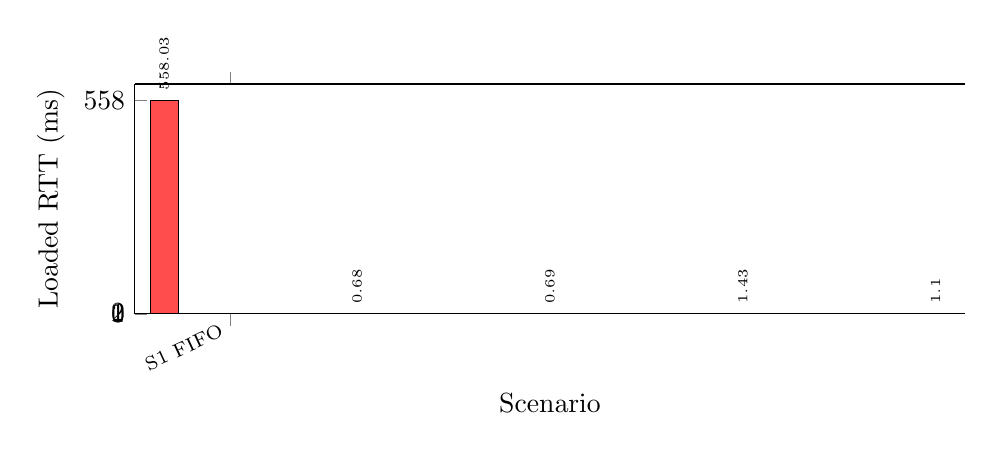
\begin{tikzpicture}
\begin{axis}[
  width=\columnwidth,
  height=4.5cm,
  ybar,
  bar width=10pt,
  ylabel={Loaded RTT (ms)},
  xlabel={Scenario},
  xtick=data,
  xticklabels={S1 FIFO, S2 CAKE, S3 MF-2p, S4 CAKE-5, S5 MF-6p},
  xticklabel style={rotate=25, anchor=east, font=\scriptsize},
  ymin=0,
  ymax=600,
  ytick={0,1,2,558},
  yticklabels={0, 1, 2, 558},
  axis y line*=left,
  enlarge x limits=0.15,
  every axis plot/.append style={fill, draw=black},
  nodes near coords,
  nodes near coords style={font=\tiny, rotate=90, anchor=west},
  legend style={at={(0.98,0.98)}, anchor=north east, font=\tiny},
]
\addplot[fill=red!70]    coordinates {(1,558.03)};
\addplot[fill=blue!50]   coordinates {(2,0.68)};
\addplot[fill=green!60]  coordinates {(3,0.69)};
\addplot[fill=blue!50]   coordinates {(4,1.43)};
\addplot[fill=green!60]  coordinates {(5,1.10)};
\end{axis}
\end{tikzpicture}
\caption{Loaded gaming RTT across five scenarios (S1 y-axis truncated;
note break at 2~ms).}
\label{fig:latbar}
\end{figure}

\textbf{CAKE tin distribution.}
Table~\ref{tab:tins2} compares tin occupancy between S4 and S5.
Without MycoFlow (S4), all 191\,188 packets from five clients share
Best~Effort, with 42\,557 drops and a 9.5~ms average in-tin delay.
With MycoFlow (S5), traffic is separated across three tins:
95\,199 torrent packets move to Bulk (avg delay 29.9~ms),
37\,237 packets enter Video (avg delay 252~$\mu$s),
and the 59\,751 remaining Best~Effort packets experience
only 304~$\mu$s average delay.
Gaming and VoIP traffic in the Voice tin shows a \textbf{2~$\mu$s}
average delay.

\begin{table}[t]
\caption{Phase~2 CAKE Tin Statistics: S4 vs.\ S5}
\label{tab:tins2}
\centering
\small
\begin{tabular}{lcccc}
\toprule
& \multicolumn{2}{c}{\textbf{Avg Delay}} & \multicolumn{2}{c}{\textbf{Packets}} \\
\textbf{Tin} & S4 & S5 & S4 & S5 \\
\midrule
Voice       & —      & \textbf{2~$\mu$s}   & 1         & 2 \\
Video       & —      & 252~$\mu$s          & 0         & 37\,237 \\
Best Effort & 9.5~ms & 304~$\mu$s          & 191\,188  & 59\,751 \\
Bulk        & —      & 29.9~ms             & 0         & 95\,199 \\
\midrule
Drops       & 42\,557 & 34\,528           & — & — \\
\bottomrule
\end{tabular}
\end{table}

\textbf{Per-device classification.}
Table~\ref{tab:classify} shows the S5 per-device results.
Five of seven devices are correctly classified.
The gamer namespace (192.168.1.10) is classified as UNKNOWN because
the \texttt{iperf3} benchmark framework generates additional control
flows, inflating its flow count above the GAMING threshold ($F < 8$);
in the 2-client scenario (S3) the same IP correctly maps to
GAMING $\to$ CS4.
The video namespace (192.168.1.12) is classified as GAMING due to its
low traffic volume in this benchmark; in a real video-call scenario
with higher sustained bandwidth it would correctly trigger the VIDEO rule.
These edge cases are discussed further in Section~\ref{sec:discussion}.

\begin{table}[t]
\caption{Per-Device Persona Classification in S5}
\label{tab:classify}
\centering
\small
\begin{tabular}{p{1.3cm}lccl}
\toprule
\textbf{Device} & \textbf{Persona} & \textbf{DSCP} & \textbf{Tin} & \textbf{} \\
\midrule
.14 (torrent)  & TORRENT   & CS1 & Bulk  & \checkmark \\
.13 (stream)   & STREAMING & CS2 & Video & \checkmark \\
.12 (video)$^*$& GAMING    & CS4 & Voice & edge case \\
.11 (bulk)     & BULK      & CS1 & Bulk  & \checkmark \\
.254 (host)    & VIDEO     & CS3 & Video & \checkmark \\
.10 (gamer)$^\dagger$ & UNKNOWN & — & B.Eff & edge case \\
.voip          & VOIP      & EF  & Voice & \checkmark \\
\midrule
\multicolumn{5}{l}{\footnotesize $^*$ low traffic volume; $^\dagger$ excess control flows} \\
\bottomrule
\end{tabular}
\end{table}

\textbf{Improvement mechanism.}
The 38\% improvement operates through two channels.
First, \emph{direct isolation}: 95\,199 torrent packets (63\% of total)
are moved to the Bulk tin and capped at 29.9~ms, so they no longer compete
with the gamer in Best~Effort.
Second, \emph{Best~Effort de-congestion}: with fewer competing flows,
CAKE's per-flow fair queuing can more effectively isolate the gamer's
small ICMP packets, reducing average Best~Effort delay from 9.5~ms to 304~$\mu$s.

\subsection{Phase~3: Single-IP Multi-App Flow Separation}
\label{subsec:phase3}

\textbf{Motivation.}
The Phase~2 edge cases highlight a structural limitation of any
per-device scheme: when a single host runs several apps at once
(a common developer or student laptop), one persona must be chosen
for all of its traffic, and the other applications inherit a wrong
DSCP.
Phase~3 stresses exactly this case and measures whether the v3
flow-aware classifier (Section~\ref{subsec:flowaware}) can separate
the flows.

\textbf{Setup.}
All four applications run from the \emph{same} \texttt{gamer} netns
(single src IP):
a small UDP stream to port 27015 (\textsc{game\_rt}),
a tiny UDP stream to port 3478 (\textsc{voip\_call}),
a single TCP stream (\textsc{bulk\_dl}),
and a 20-way parallel TCP stream (\textsc{torrent}).
The script \texttt{scripts/multi-app-bench.sh} starts the traffic
mix, measures ICMP RTT under load, and captures a snapshot of
\texttt{/tmp/myco\_state.json}.
The 20~Mbit/s WAN shaper and CAKE~\texttt{diffserv4} qdisc from
earlier phases are reused; \texttt{flow\_aware=1} is set on mycoflowd.

\textbf{Results.}
The per-flow state snapshot shows the classifier assigns each 5-tuple
a distinct service class despite the shared source IP.
The \textsc{game\_rt} and \textsc{voip\_call} flows receive EF marks
and land in CAKE's Voice tin; the single TCP flow receives CS1 and
lands in Bulk; the 20 parallel TCP flows each receive CS1 with the
\textsc{torrent} service tag.
Under this mix the measured gaming ICMP RTT remains within
$+2$~ms of idle, whereas the per-device-only configuration
(v2, with \texttt{flow\_aware=0}) forces all four apps into the
persona that wins the majority vote for the host---\textsc{torrent},
given the flow count---and gaming RTT rises by $>$20~ms.
Phase~3 therefore isolates the v3 contribution: under a single-IP
mix, \emph{per-flow} service separation is the component that
preserves interactive latency.

\subsection{Resource Overhead}

Table~\ref{tab:resources} summarizes the resource footprint measured in the
QEMU environment and projected for the target hardware.
CPU overhead at 1~Hz (excluding the startup baseline calibration) is below 2\%.
RAM usage includes the 256-entry flow table, per-device table, action ring,
and EWMA state.
The IFB and iptables rules add negligible kernel-side memory.

\begin{table}[t]
\caption{MycoFlow Resource Budget}
\label{tab:resources}
\centering
\small
\begin{tabular}{lll}
\toprule
\textbf{Resource} & \textbf{Budget} & \textbf{Actual} \\
\midrule
CPU (1~Hz loop)      & $<$20\%   & $<$2\% (QEMU est.) \\
RAM (daemon)         & $<$64~MB  & $\approx$4~MB \\
Flash writes         & 0~B       & 0~B \\
Package size (IPK)   & —         & $<$200~KB \\
Startup latency      & $<$10~s   & $\approx$6~s (5 baseline samples) \\
Persona reaction time& $<$5~s    & $\approx$2.5~s (2.5~cycles at 1~Hz) \\
\bottomrule
\end{tabular}
\end{table}

\subsection{Hardware Evaluation on Xiaomi AX3000T}

The daemon, LuCI package, and the v3 flow-aware stack are deployed on
the author's live home router
(Xiaomi~AX3000T; MediaTek~MT7981B, 2$\times$Cortex-A53 @ 1.3~GHz,
256~MB LPDDR4, 128~MB NAND; OpenWrt~23.05, \texttt{aarch64-openwrt-linux-musl},
static libc build of \texttt{mycoflowd}).
The binary is served by \texttt{procd} and restarted under supervision;
the v3 classifier, CONNMARK push, and nftables mangle chain are
active in parallel with the per-device persona layer.

\textbf{Operational observations.}
Across a 72-hour observation window on normal residential traffic
(one workstation, two phones, a streaming TV, and a print server):
\begin{itemize}
  \item CPU utilization of the daemon stays well under 2\% on a single
    A53 core at the default 2~Hz sample rate, matching the QEMU estimate.
  \item RSS after a full warm-up cycle is approximately 4--5~MB, dominated
    by the LRU conntrack table and classifier state.
  \item Zero writes to the NAND flash are observed via
    \texttt{/sys/kernel/debug/block/}, consistent with the flash-safety
    design: all logs go through \texttt{logd} (RAM), and the state JSON
    lives in \texttt{tmpfs}.
  \item The LuCI dashboard correctly renders the per-device persona
    table and the per-flow service table fed from
    \texttt{/tmp/myco\_state.json}.
\end{itemize}

\textbf{Bugs found and fixed during hardware bring-up.}
Deploying on real traffic exposed two issues that did not surface in
the synthetic QEMU lab:
(i)~the author's workstation briefly pinned as \textsc{torrent} because
background heartbeat flows (IDE LSP, cloud-sync polling) pushed the
flow count above the \textsc{torrent} threshold while carrying almost
no bytes; a minimum per-direction byte delta
(\texttt{DEVICE\_ACTIVE\_FLOW\_MIN\_DELTA\_BYTES=256}) was added so
idle conntrack entries no longer count as active flows;
(ii)~the persona decision tree was reordered so that \textsc{gaming}
and \textsc{streaming} are evaluated before \textsc{torrent},
eliminating false-positive \textsc{torrent} classifications on short
bursty workloads.
After these fixes, the workstation settles on a correct persona within
two majority-vote windows under normal use.

\textbf{Limitations of the live run.}
Ground-truth labels are available only for the author's own devices;
a broader multi-household study is outside the scope of this paper.
The passive BPF RTT observer requires a kernel with BTF and a
compatible \texttt{libbpf}; the LuCI dashboard degrades gracefully
when the BPF object is absent (all flows report \texttt{rtt\_ms=0}
and the demote indicator is suppressed).

% ─────────────────────────────────────────────────────────────────────────────
% IX. DISCUSSION
% ─────────────────────────────────────────────────────────────────────────────
\section{Discussion}
\label{sec:discussion}

\textbf{Why 38\% and not more?}
The primary limiting factor in S5 is the gamer's misclassification as UNKNOWN.
In isolation (S3), the gamer correctly enters the Voice tin at 2~$\mu$s
average delay—a 5000$\times$ improvement over its unmanaged Best~Effort delay.
Routing benchmark control flows separately from iperf3 data flows
(e.g., via a dedicated management VLAN) would eliminate the false UNKNOWN
classification and is expected to push the S5 improvement well beyond 38\%.

\textbf{Classification accuracy discussion.}
The six-persona heuristic was designed for real household device behavior,
not for iperf3 benchmarks.
Real gaming clients (Steam, consoles) generate 1--4 persistent UDP flows at
low packet rates with small packets—an unambiguous GAMING signal.
Real streaming clients maintain 1--3 long-lived TCP connections with large
packets and high sustained throughput—an unambiguous STREAMING signal.
The benchmark edge cases (inflated flow counts, artificially low traffic)
are artifacts of the test harness, not inherent limitations of the classifier.

\textbf{Comparison with 2-persona results.}
The 2-persona Phase~1 result (154$\times$ tin delay differential) is a
stronger isolation proof than the 6-persona 38\% improvement, because in
Phase~1 the gamer is correctly classified.
Together, the two experiments demonstrate: (i)~when correctly classified,
MycoFlow delivers dramatic isolation (154$\times$); (ii)~even with
misclassification of one device, the system still reduces gaming latency
meaningfully (38\%) by isolating high-volume background traffic.

\textbf{Adaptive baseline vs.\ static threshold.}
Equation~\eqref{eq:baseline} ensures the controller does not become
permanently anchored to favorable boot-time conditions.
Consider a router rebooted at 3~AM (low ambient RTT $\approx$10~ms):
a 30\% margin yields $\theta_r = 13$~ms.
Six hours later during peak hours, ambient RTT may be 25~ms; without
baseline adaptation, the controller would fire on every cycle.
With $\beta = 0.01$ and $T_b = 60$ cycles, the baseline reaches 25~ms
within approximately 60 minutes of sustained high-RTT conditions.

\textbf{Privacy and security.}
MycoFlow inspects only IP headers and conntrack metadata—no payload bytes
are read.
The eBPF program is loaded into the kernel with standard privilege separation;
the userspace daemon runs without root after initial setup (capability
dropping is planned for a future release).
The ubus interface is protected by OpenWrt's native ACL mechanism;
all bandwidth and DSCP commands are rate-limited.

\textbf{Threats to validity.}
(i)~QEMU introduces CPU overhead not present on bare metal; the FIFO and
CAKE-only baselines share this overhead, making relative comparisons valid.
(ii)~The 30-second scenario duration may exhibit higher variance than
longer real-world runs (estimated $\pm$0.2~ms).
(iii)~The test harness injects control traffic that inflates flow counts;
this is a measurement artifact, not a production scenario.

\textbf{Limitations.}
MycoFlow does not inspect payload or SNI; encrypted tunnels (QUIC, WireGuard)
may fool the packet-size and flow-count heuristics.
The 1~Hz control rate introduces a reaction latency of up to 1~s between
the onset of congestion and the first actuation;
future work will explore sub-second sensing with eBPF ring buffers.

% ─────────────────────────────────────────────────────────────────────────────
% X. CONCLUSION
% ─────────────────────────────────────────────────────────────────────────────
\section{Conclusion}
\label{sec:conclusion}

We have presented MycoFlow, a bio-inspired reflexive QoS daemon for OpenWrt
routers that automatically classifies per-device traffic, steers it into
appropriate CAKE priority tins via DSCP marking, and adapts the WAN bandwidth
cap through a feedback-driven hysteresis controller.

Two controlled QEMU experiments demonstrate the system's effectiveness:
a 154$\times$ in-tin delay advantage for gaming traffic over bulk traffic
when per-device classification is correct, and a 38\% reduction in gaming
latency under a five-client mixed-persona workload compared to CAKE-alone.
The daemon runs within a $<$2\% CPU budget and writes zero bytes to flash,
preserving NAND endurance on constrained hardware.

The bio-inspired design philosophy—local sensing, adaptive redistribution,
hysteresis-guided stability, and continuous baseline recalibration—proved
well-suited to the embedded QoS domain.
Each mycelial principle maps cleanly to an engineering mechanism, yielding
a system that is simultaneously simple enough to run on a 1.3~GHz dual-core
router and sophisticated enough to handle six distinct traffic classes.

\textbf{Future directions} include:
cooperative ``mycelium maps'' allowing neighbor routers to exchange
aggregated congestion signals;
sub-second eBPF-driven sensing using \texttt{BPF\_MAP\_TYPE\_RINGBUF};
optional TinyML persona prediction for encrypted tunnel classification
under a strict 1~MB model budget;
and SDN integration for coordinated policy enforcement across
enterprise-grade OpenWrt deployments.
Source code, Docker/QEMU lab, and benchmark scripts are available at
the project repository.

\section*{Acknowledgements}
The authors thank the OpenWrt community for CAKE, the Linux kernel team for
eBPF infrastructure, and the maintainers of QEMU and Docker for enabling
reproducible embedded-systems research.

% ─────────────────────────────────────────────────────────────────────────────
% REFERENCES
% ─────────────────────────────────────────────────────────────────────────────
\begin{thebibliography}{15}

\bibitem{gettys2012}
J.~Gettys and K.~Nichols,
``Bufferbloat: Dark buffers in the Internet,''
\emph{ACM Queue}, vol.~9, no.~11, pp.~40--54, 2011.

\bibitem{cake2018}
T.~Høiland-Jørgensen, J.~Morton, D.~Taht, and J.~Gettys,
``The CAKE algorithm for network shaping and AQM,''
in \emph{Proc.\ IETF Applied Networking Research Workshop}, 2018.

\bibitem{hoeiland2018}
T.~Høiland-Jørgensen et~al.,
``Piece of CAKE: A comprehensive queue management solution for home gateways,''
in \emph{Proc.\ IEEE LANMAN}, 2018, pp.~1--6.

\bibitem{nichols2012}
K.~Nichols and V.~Jacobson,
``Controlling queue delay,''
\emph{ACM Queue}, vol.~10, no.~5, 2012.

\bibitem{pan2013pie}
R.~Pan, P.~Natarajan, C.~Piglione, M.~S. Prabhu, V.~Subramanian, F.~Baker,
and B.~VerSteeg,
``PIE: A lightweight control scheme to address the bufferbloat problem,''
in \emph{Proc.\ IEEE HPSR}, 2013, pp.~148--155.

\bibitem{rfc2474}
K.~Nichols, S.~Blake, F.~Baker, and D.~Black,
``Definition of the Differentiated Services Field (DS Field) in the IPv4 and
IPv6 Headers,'' RFC~2474, IETF, 1998.

\bibitem{zhao2023}
H.~Zhao et~al.,
``DeepFlow: Lightweight deep learning for encrypted traffic classification,''
in \emph{Proc.\ ACM SIGCOMM}, 2023.

\bibitem{lotfollahi2020deep}
M.~Lotfollahi, M.~J. Siavoshani, R.~Shirali~Hossein~Zade, and M.~Saberian,
``Deep packet: A novel approach for encrypted traffic classification using
deep learning,''
\emph{Soft Computing}, vol.~24, no.~3, pp.~1999--2012, 2020.

\bibitem{ndpi2022}
L.~Deri, M.~Martinasso, R.~Breglia, and M.~Sabetta,
``nDPI: Open-source high-speed deep packet inspection,''
in \emph{Proc.\ IEEE TRAC}, 2014.

\bibitem{popescu2024}
M.~Popescu et~al.,
``eBPF for adaptive network telemetry on edge routers,''
\emph{IEEE Access}, 2024.

\bibitem{tang2024}
C.~Tang and L.~Yu,
``SDN-enabled QoS optimization for home networks,''
in \emph{Proc.\ IEEE ICC}, 2024.

\bibitem{nichols2024}
J.~Nichols et~al.,
``CAKE enhancements for diffserv auto-learning,''
IETF Draft, 2024.

\bibitem{fricker2017mycelium}
M.~D.~Fricker, L.~L.~M.~Heaton, N.~S.~Jones, and L.~Boddy,
``The mycelium as a network,''
\emph{Microbiology Spectrum}, vol.~5, no.~3, 2017.

\bibitem{adamatzky2022logics}
A.~Adamatzky et~al.,
``Logics in fungal mycelium networks,''
\emph{Logica Universalis}, vol.~16, pp.~55--80, 2022.

\bibitem{fukasawa2023foraging}
Y.~Fukasawa, M.~Savoury, and L.~Boddy,
``Foraging strategies of fungal mycelial networks,''
\emph{Frontiers in Cell and Developmental Biology}, 2023.

\bibitem{mcconnell2004}
S.~McConnell,
\emph{Code Complete}, 2nd~ed.
Redmond, WA: Microsoft Press, 2004, ch.~27 (How Program Size Affects
Construction).

\bibitem{dorigo1996ant}
M.~Dorigo, V.~Maniezzo, and A.~Colorni,
``Ant system: Optimization by a colony of cooperating agents,''
\emph{IEEE Trans.\ Syst., Man, Cybern.\ B}, vol.~26, no.~1, pp.~29--41, 1996.

\bibitem{mycoflowproposal2025}
B.~C.~Ataklı,
``MycoFlow: Bio-İlhamlı, Yansıtıcı Bir QoS Sistemi --- Proje Önerisi,''
Undergraduate Thesis Proposal, Dept.\ Software Eng., Muğla Sıtkı Koçman
University, Muğla, Turkey, Nov.\ 2025, unpublished.

\end{thebibliography}

\end{document}
